%\documentclass{article}
%\usepackage{verbatim}
%\usepackage{graphicx}
%\usepackage{amssymb,amsmath}
%usepackage{multirow}

\section{Level 1: How to run your first simulation with RUMD }

%\author{LB}
%\date{Level 1}

%\begin{document}
%\maketitle

This tutorial assumes basic GNU/Linux knowledge, a successful
installation of RUMD and a little portion of gumption mixed
with interest in molecular dynamics. For plotting the results 
from simulations it is assumed that xmgrace is installed, but 
other plotting programs can be used if you prefer. 

The basic work-flow of doing simulations is:
\begin{itemize}
  \item Specify initial condition, i.e., the initial positions 
        and velocities to be used in the simulation. This also involves
        the number of particles ($N$) and the (initial) density 
        ($\rho\equiv N/V$).
  \item Running the actual simulation. This can be done interactively 
        or by a script in python. It includes defining how particles 
        interact with each other (i.e., the potentials used), what 
        integrator to use (and the associated parameters, e.g., 
        time-step and temperature.)
  \item Post-processing data analysis.
\end{itemize}
The following sub-sections will take you through these steps.

\subsection{The initial condition}

When conducting simulations it is often convenient to use the end result 
of one simulation as the initial condition to a new simulation.
However, sometimes you need to generate a fresh initial condition. 
This can be done from a terminal window by executing the commands given below. 

First make a directory where you want your first simulation to be performed. Call
it e.g. \verb=~/Test/=, and go to that directory:
\begin{verbatim}
mkdir Test
cd Test
\end{verbatim}
Next, run the \verb=rumd_init_conf= program (make sure  \verb=RUMD_home/Tools/= is 
in your path):
\begin{verbatim}
rumd_init_conf --lattice=fcc --cells=6
\end{verbatim}
This command produces a file called \verb|start.xyz.gz| that we will use as the initial configuration. 
The flag \verb|--lattice=fcc| tells the program to generate a fcc crystal, and 
the flag \verb|--cells=6| that is should make six unit cells in each direction.
The fcc lattice have four particles in the unit cell, and the final configuration
will have $4\times6^3=864$ particles.
%
We have not specified a density or temperature to the program, 
and it will use default values of $\rho=1.0$ and $T=1.0$, respectively. 
Note that \verb|rumd_init_conf| have many options for generating configurations.
A summary of these can be seen by typing
\begin{verbatim} 
rumd_init_conf --help
\end{verbatim}
\verb|rumd_init_conf| also accept ``short arguments'' and the command to generating 
the fcc lattice simply done with
\begin{verbatim}
rumd_init_conf -lfcc -c6
\end{verbatim}

\newlength{\saveparindent}
\setlength{\saveparindent} {\parindent}
\setlength{\parindent}{0 pt}

\subsection{Executing your first program using the python interface}
%
In this first example we will simulate a single component
Lennard--Jones liquid. We will work with python interactively, so that you can
 get a feel for what is possible. For production runs you will normally
make a script containing the appropriate python commands. Start python by typing
\begin{verbatim}
python3
\end{verbatim}
in a terminal. You will get a python prompt that looks like 
``\verb|>>>|''. Type 

\verb|  from rumd import * |

This will import the main RUMD classes into the
global namespace\footnote{Alternatively (recommended by some to avoid possible name clashes in the global namespace) one can type \texttt{import rumd}, and then all of the class-names, etc., must be prefixed by \texttt{rumd.}, for example \texttt{rumd.IntegratorNVE}.} (these are actually C++ classes, but we can ``talk'' to them through python). These are in principle enough to write scripts and thereby run simulations, but to simplify this process, there is an extra python
class called \verb|Simulation|: type
 
\verb|  from rumd.Simulation import Simulation|

This class combines access to the main data-structures 
with the main integration loop and various functions for controlling output 
etc. To start a simulation we first 
create a \verb|Simulation| object, passing the 
name of a starting configuration file:

\verb|  sim = Simulation("start.xyz.gz")|

Here \verb|sim| is an arbitrary name we choose for the object.
Next we choose an NVT integrator, giving the time-step,  temperature and the relaxation time controlling the thermostat [RUMD versions before 3.4 did not require the latter to be explicitly set and set a default value of 0.2]:

\verb|  itg = IntegratorNVT(timeStep=0.0025, targetTemperature=1.0, thermostatRelaxationTime=0.2)|

Having an integrator object, we need to connect it to the simulation:

\verb|  sim.SetIntegrator(itg)|

Next we need to choose the potential. For 12-6 Lennard-Jones we create a 
potential object, giving it the name \verb|pot|, as follows:

\verb|  pot = Pot_LJ_12_6(cutoff_method=ShiftedPotential)|
 
The mandatory argument \verb|cutoff_method| specifies how the cut-off of
the pair-potential is to be handled. It must be one of
\verb|ShiftedPotential| (the most common method, where the potential is
shifted to zero), \verb|ShiftedForce| or \verb|NoShift|
We need to set the parameters, which is done using the method \verb|SetParams|.
The arguments to this method depend on which potential class you are
working with, but they can be found by typing

\verb|  help(pot.SetParams)|

which displays a help page generated from the ``docstring'' of the method
(alternatively type \verb|print pot.SetParams.__doc__|).
In particular this includes a list of the arguments:

\begin{verbatim}
  SetParams(self, unsigned int i, unsigned int j, float Sigma, 
  float Epsilon, float Rcut)
\end{verbatim}


The first one, \verb|self|, represents the object itself, and is not explicitly
given when calling the function. The next two define which particle types we
are specifying parameters for---we just have one type of particle so both will
be zero; the two after that are the standard Lennard-Jones length and energy
parameters, while the last is the cut-off in units of Sigma. Press Q to exit
the help screen. We choose the following:

\verb|  pot.SetParams(0, 0, 1.0, 1.0, 2.5)|

Note that we can also use python's ``keyword arguments'' feature to specify the
arguments, which can then be in any order, for example:

\verb|  pot.SetParams(i=0, j=0, Epsilon=1.0, Rcut= 2.5, Sigma=1.0)|

The potential also needs to be connected to the simulation:

\verb|  sim.AddPotential(pot)|

[The old function \verb|SetPotential| is deprecated as of Version 3.5] Now we are ready to run a simulation. To run a simulation with 20000 time steps,
we just write

\verb|  sim.Run(20000)|

Various messages will be printed to the screen while it is running (these can
 be turned off with \verb|sim.SetVerbose(False)|. If we like, we
can get the positions after the 20000 steps by getting them as a numpy array 
(numpy, or numerical python, is a package that provides efficient array-based
numerical methods), and in particular look at the position of particle 0 by typing

\begin{verbatim}
  pos = sim.sample.GetPositions()
  print pos[0]
\end{verbatim}

However more likely we will run an analysis program on the output
files produced by the simulation during the operation of the \verb|Run|
function. The available analysis programs are described below in subsection~ 
\ref{postProcessing} in their command-line forms. Some of them (eventually all)
can also be called from within python. 
For now let's write a configuration file for possible use as a starting point
for future simulations. Here we go a little deeper into the interface.
Objects of type \verb|Simulation| have an attribute
called "sample" of type Sample 
(the main C++ class representing the sample we are simulating). We call its
\verb|WriteConf| method as follows:

\verb|  sim.WriteConf("end.xyz.gz")|


Type Ctrl-D to exit python. Next we would like to make scripts. Here is the 
script that contains the 
commands we have just worked through (the lines starting with \verb|#|
are comments):


% \begin{lstlisting}[language=python]
% \begin{minted}{python}
\begin{verbatim}
  from rumd import *
  from rumd.Simulation import Simulation

  # create simulation object
  sim = Simulation("start.xyz.gz")

  # create integrator object
  itg = IntegratorNVT(timeStep=0.0025, targetTemperature=1.0, thermostatRelaxationTime=0.2)
  sim.SetIntegrator(itg)

  # create potential object
  pot = Pot_LJ_12_6(cutoff_method=ShiftedPotential)
  pot.SetParams(0, 0, 1.0, 1.0, 2.5)
  sim.AddPotential(pot)

  # run the simulation
  sim.Run(20000)

  # write final configuration
  sim.WriteConf("end.xyz.gz")
\end{verbatim}
% \end{minted}
% \end{lstlisting}


If this script is saved as a file called, for example, run.py (it must end in
.py), then it is run by typing
\verb|python3 run.py|. This will exit python when finished. To leave python on
after the script has completed, type \verb|python3 -i run.py| (-i means run in
interactive mode). If it is to be run on a batch queue, the appropriate PBS
commands should be included in comments at the top as follows:

\begin{verbatim}
  #!/usr/bin/python3
  # pass PYTHONPATH environment variable to the batch process
  #PBS -v PYTHONPATH
  #PBS (other PBS commands here)
  #PBS 
  #PBS 

  # this ensures PBS jobs run in the correct directory
  import os, sys
  if "PBS_O_WORKDIR" in os.environ:
      os.chdir(os.environ["PBS_O_WORKDIR"])
      sys.path.append(".")


  from rumd import *
  (etc)
\end{verbatim}

It should be submitted using \verb|qsub run.py|. Note that the 
indentation of the two lines following the \verb|if| statement is important!

\subsection{Setting options with the python interface}

Here we present some of the options available for controlling simulations.

\subsubsection{Choosing the potential and its parameters}

Probably the most important thing a user needs to control is the 
potential. Different potentials are represented by different classes; objects
are created just as above, so for example:

\begin{verbatim}
  # generalized LJ potential (here m=18, n=4)
  potential = Pot_gLJ_m_n(18,4, cutoff_method=ShiftedPotential) 
  # inverse power-law (IPL) with exponent n=12
  potential = Pot_IPL_12(cutoff_method=ShiftedPotential)
\end{verbatim}


To set parameters for the potential, call its \verb|SetParams| method as 
described above. If a binary system is to be simulated, 
the parameters should be set separately for each interaction pair as follows

\begin{verbatim}
  potential.SetParams(0, 0, 1.00, 1.00, 1.12246)
  potential.SetParams(0, 1, 0.80, 1.50, 1.12246)
  potential.SetParams(1, 1, 0.88, 0.50, 1.12246)
\end{verbatim}

Note that Newton's third law is assumed to hold, so setting the parameters for 
i=0 and j=1 automatically sets those for i=1 and j=0 (we could also have 
called \verb|SetParams| with the latter).
An overview of the available potentials is given in the user manual. 

\subsubsection{Choosing the integrator}

Perhaps the next most important choice is what kind of integration algorithm
to use. Above we did a constant-temperature (NVT) algorithm (the actual
algorithm is of the Nos{\'e}-Hoover type). For constant energy (NVE) runs we
create the integrator as follows, here passing only the time-step:

\verb|itg = IntegratorNVE(timeStep=0.0025)|

(Technical note: this creates an object of the same type as IntegratorNVT,
but here it defaults to NVE mode---in fact in either case one can switch 
thermostatting on or off using the \verb|SetThermostatOn()| method). 

\newlength{\parwidth}
\setlength{\parwidth}{6 cm}


Additional integrators available in RUMD are listed below
\newline \newline
\begin{tabular}{ | l | c | c |}
  \hline  
  \hline
  Name of Integrator & \textbf{Description} & Arguments \\
  \hline
  IntegratorNVE & \parbox{\parwidth}{The \textit{NVE} Leap-frog algorithm.} & \verb=timeStep= \\
  IntegratorNVT & \parbox{\parwidth}{The Nos$\acute{e}$-Hoover \textit{NVT} algorithm.} & \verb=timeStep, targetTemperature, thermostatRelaxationTime= \\
  IntegratorNPTAtomic & \parbox{\parwidth}{\textit{NPT} algorithm. (JCP 101, N 5, 1994)} & \parbox{\parwidth}{ \centering \Q{timeStep, targetTemperature, thermostatRelaxationTime, targetPressure, barostatRelaxationTime} } \\
  IntegratorNVU & \parbox{\parwidth}{Algorithm conserving the total potential energy.} & \verb=dispLength, potentialEnergy= \\
  IntegratorMMC & \parbox{\parwidth}{Metropolis \textit{NVT} Monte Carlo.} & \verb=dispLength, targetTemperature= \\
  IntegratorIHS &\parbox{\parwidth}{ Energy minimization via the Leap-frog algorithm.} & \verb=timeStep= \\
  IntegratorSLLOD & \parbox{\parwidth}{Shear an atomic system in the xy-plane using the SLLOD equations.} & \verb=timeStep, strainRate= \\
  IntegratorMolecularSLLOD & \parbox{\parwidth}{Shear a molecular system in the xy-plane using the SLLOD equations.} & \verb=timeStep, strainRate= \\ 
IntegratorNPTLangevin & \parbox{\parwidth}{Algorithm which generates the \textit{NPT} ensemble using Langevin dynamics} & \verb=timeStep, targetTemperature, friction, targetPressure, barostatFriction, barostatMass= \\
  \hline
  \hline
\end{tabular}
\newline \newline
The above integrators are chosen in the usual way with named arguments as given in the table.
In the case of IntegratorNPTAtomic the user must choose suitable relaxation times for the thermostat and the barostat.
An example of reasonable values for the thermostat and barostat relaxation times for the LJ system at $T=2.0$ and $p=5.0$ are 
\Q{thermostatRelaxationTime=0.4} and \Q{barostatRelaxationTime=10.0}. For IntegratorNPTLangevin the friction may be chosen over a wide range, depending on how strongly individual particles should be coupled to the heat bath. For the box dynamics, note that the ratio of barostatMass to barostatFriction is a relaxation time which should be reasonable for the system (at least long compared to the time step).

\subsubsection{Controlling how frequently to write output}

To control the output written to files we use the \verb|Simulation|
method \verb|SetOutputScheduling|. By default there are two ``output
managers'': ``energies'' and ``trajectory''. The first is for the files 
containing potential/kinetic energies and other global
quantities, while the second is for trajectories (configuration files 
containing the particle positions at different times during the run). 
The write-schedule for either manager
can be evenly-spaced in time (``linear''), 
logarithmic (``logarithmic''), or a  kind of combination of the two 
(``loglin''). Examples of controlling scheduling include

\begin{verbatim}
  sim.SetOutputScheduling( "energies", "linear", interval=50)
  sim.SetOutputScheduling( "energies", "none" )
  sim.SetOutputScheduling( "trajectory", "logarithmic" )
  sim.SetOutputScheduling( "trajectory", "loglin", base=4, maxInterval=64 )
\end{verbatim}

The first causes energies to be output equally spaced (linear) in time, once 
every 50 time steps, while the second turns energy writing off. The third
 will cause logarithmic saving of configurations (where the 
interval between saves doubles 
each time within a ``block'', starting with 1. The fourth does
logarithmic saving starting with interval 4 until the interval 64 is
reached, after which the interval stays fixed at 64 until the end of
the block. The details of log-lin  are described in a separate
document.  By default energies are linear, written every 256 steps,
and trajectories are logarithmic.  


\subsection{\label{postProcessing} Post processing}

The post processing tools are located in the \verb=<RUMD-HOME>/Tools/=
directory and each one of them has a help text. To see the help text
use the option \verb|-h| or \verb|--help| depending on the tool. 
The actual output files generated by the program are in a
directory called \verb|TrajectoryFiles|. When you start a new simulation in the
same directory, this will be moved to \verb|TrajectoryFiles.rumd_bak| as 
a precaution against accidental overwriting of data. The analysis 
programs should be run in the original directory where the simulation was run
(they know they should look in \verb|TrajectoryFiles| for the data).


\verb=rumd_stats= produces mean values, variances and standard
deviations for specific quantities. The \verb=rumd_stats= stdout for
the simulation just performed is shown in table \ref{stat}.  
\begin{table}[!ht]
  \begin{center}
    \begin{tabular}{ l r r r }
      quantity & mean value &  variance & standard deviation \\
      ke     &  1.49802	  &  0.0015541	 &  0.0394221 \\
      pe     & -5.27922	  &  0.0029679	 &  0.0544784 \\
      p	     &  8.64558	  &  0.0529826	 &  0.23018 \\
      T	     &  0.999677  &  0.000692101 &  0.0263078 \\
      Etot   & -3.7812	  &  0.00439295	 &  0.0662794 \\
      W	     &  7.64591	  &  0.052637	 &  0.229428 \\
      \label{stats}
    \end{tabular}
    \caption{rumd\_stats output.}\label{stat}
  \end{center}
\end{table}

Here ke is the kinetic energy, pe is the potential energy, p is the
pressure, T is the kinetic temperature, Ps is the Nose Hoover
thermostat, Etot is the total kinetic energy and W is the virial. The
program writes the mean and variance in the files
\verb=energies_mean.dat= and \verb=energies_var.dat= in one row as the
first column of stdout. 

The radial distribution function is computed by typing 
\verb=rumd_rdf -n 1000 -m 1.0= 
where the first argument is the number of bins in radial
distribution function and the second argument, the minimum time
between successive configurations to use, is to avoid wasting 
time doing calculations that are very similar (we assume here that the
 configurations are  uncorrelated after one time unit). Use
 \verb|rumd_rdf -h| for a full list of arguments. 
The output is \verb=rdf.dat= and for binary systems the columns are:\\
$r \quad g_{00}(r) \quad  g_{01}(r)\quad  g_{10}(r)\quad
g_{11}(r)$. (Single component only has two columns). Plot
\verb=rdf.dat= to obtain figure \ref{rdf}.  
\begin{figure}[!ht]
  \centering
  \includegraphics[scale=0.3]{level1/LJrdf.eps}
  \caption{Radial distribution function.}\label{rdf}
\end{figure}

The static structure factor can be obtained when the radial
distribution function is computed. It is done by typing 
\verb=rumd_sq 2 20 1= 
where the first argument is the start $q$ value, the second
argument is the final $q$ value and the third argument is the
density. The stdout is the $q$ value for the maximum of the first peak
and it is written in a file called \verb=qmax.dat=. The static
structure factor is written in \verb=Sq.dat= and is structured like
\verb=rdf.dat=. Plot \verb=Sq.dat= to obtain figure \ref{LJSq}.\\ 
\begin{figure}[!ht]
\centering
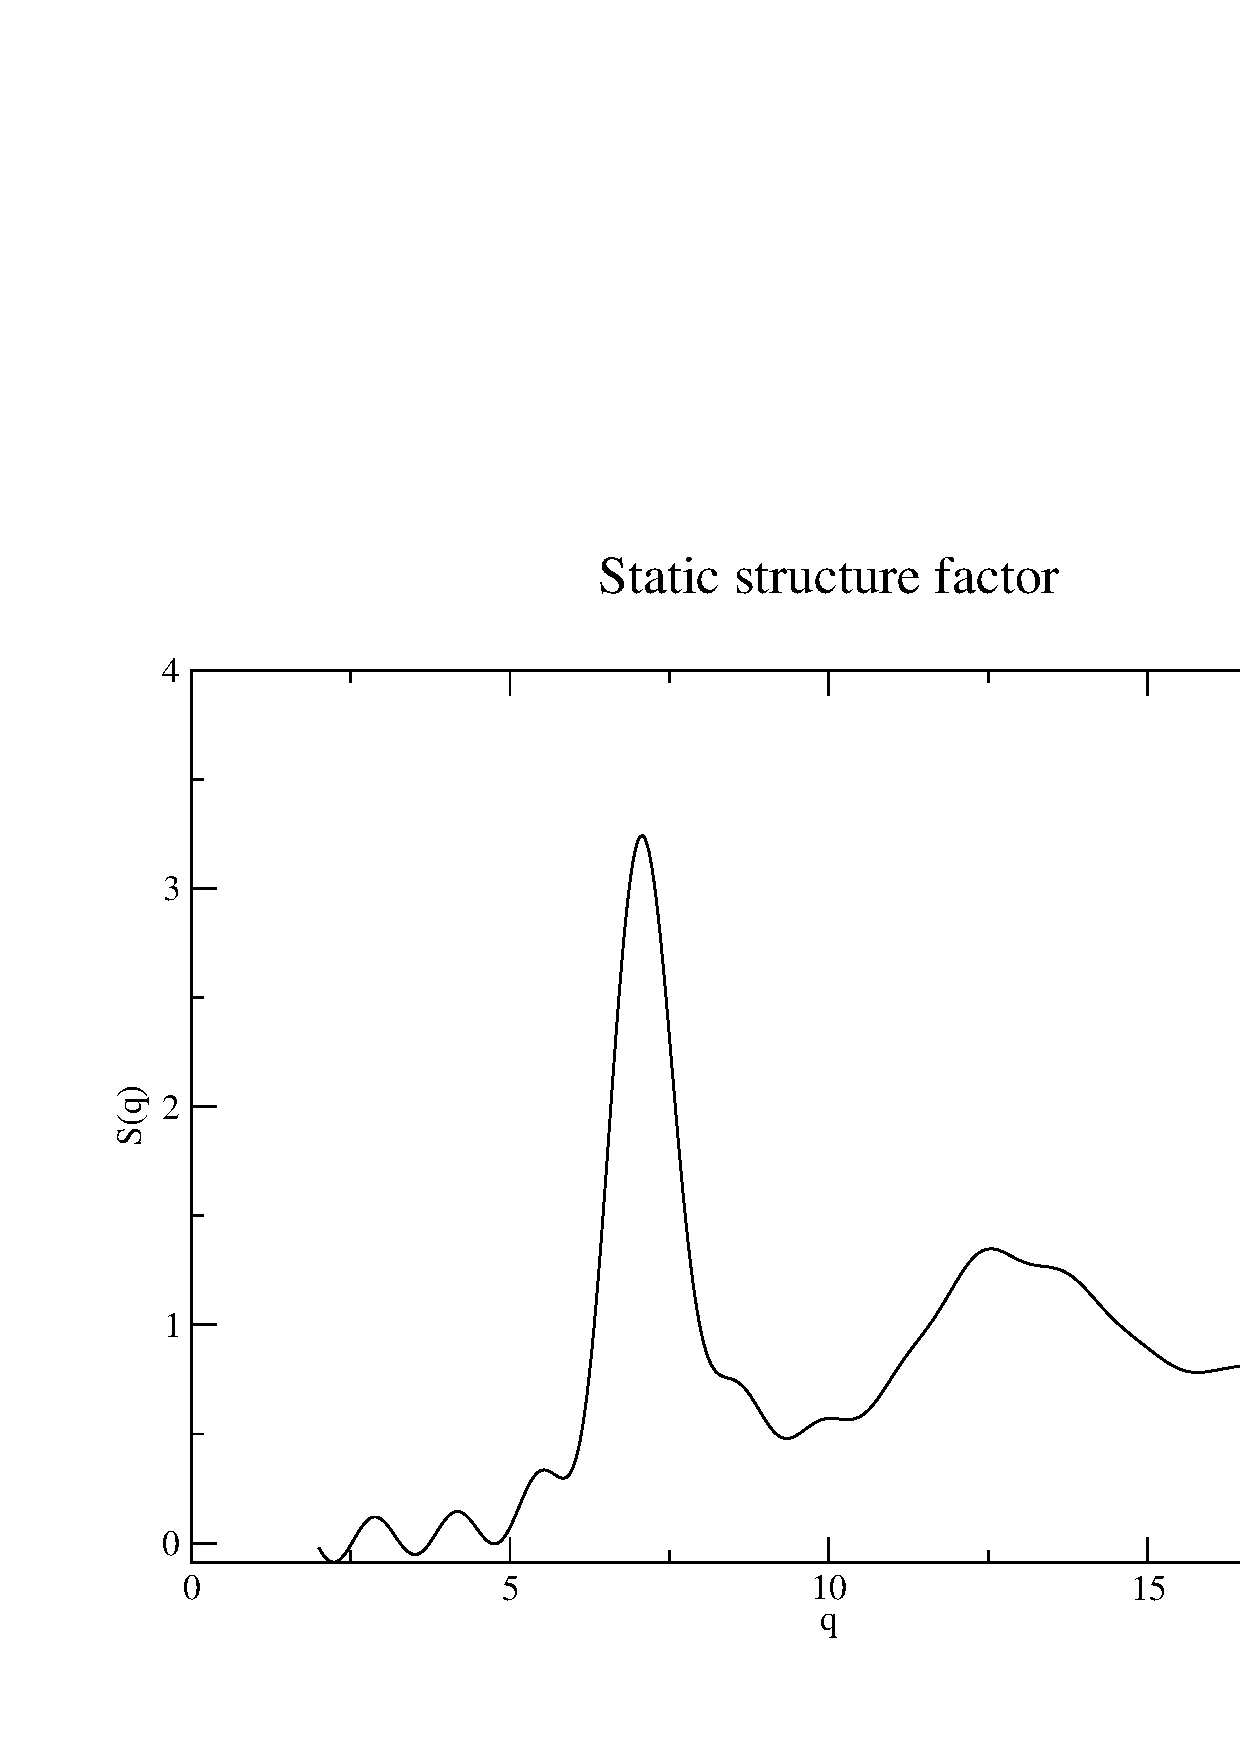
\includegraphics[width=0.6\textwidth]{level1/LJSq}
\caption{The static structure factor}\label{LJSq}
\end{figure}
The mean square displacement and the self part of the
incoherent intermediate scattering function $F_q(t)$ are calculated with 
the command
\verb=rumd_msd=. This generates a \verb=msd.dat= file with time as the
first column and the mean square displacement as a function of time as
the second column (for binary systems there will be two columns), and a file 
\verb|Fs.dat| with a similar structure. Before it can
be run however, you must create a file called \verb|qvalues.dat| which contains
one wavenumber for each type of particle. Typically these correspond to the 
location of the first peak in the structure factor, so one could copy the file
\verb|qmax.dat| created by \verb|rumd_sq|. \verb|rumd_msd| also calculates
gaussian parameter \verb=alpha2.dat=. See figure \ref{msd} and
\ref{Fs} for mean square displacement and self part of incoherent
scattering function.
\begin{figure}[!ht]
\centering
\includegraphics[width=0.6\textwidth]{level1/LJmsd}
\caption{Mean square displacement.}\label{msd}
\end{figure}
\begin{figure}[!ht]
\centering
\includegraphics[width=0.6\textwidth]{level1/LJFs}
\caption{Self part of the intermediate scattering function evaluated
  at the $q$ value of the maximum of the first peak in the structure
  factor.}\label{Fs} 
\end{figure}
The post processing analysis tools are summarized in table \ref{pp}.
 \begin{table}
   \begin{center}
  \begin{tabular}{l c c r}
  \hline \hline
  Tool & Input & Output & Arguments\\
  \hline
  \multirow{3}{*}{rumd\_stats}
   &  & std.out: table \ref{stat} &  \\
   & none & energies\_mean.dat & none \\
   & & energies\_var.dat &  \\
  \hline
  \multirow{3}{*}{rumd\_rdf}
   &  & std.out: Simulation info & 1. num. bins \\
   & none & rdf.dat & 2. time diff. \\
   &  & sdf.dat &  \\
  \hline
  \multirow{3}{*}{rumd\_sq}
   &  & std.out: qmax(s) & 1. qstart \\
   & rdf.dat & Sq.dat & 2. qfinal \\
   &  & qmax.dat & 3. density \\
  \hline
  \multirow{5}{*}{rumd\_msd}
   &  & std.out: Simulation info & \\
   &  & msd.dat  & \\
   & qvalues.dat &  Fs.dat & none\\
   &  &  FsSq.dat & \\
   &  &  alpha2.dat & \\
  \hline \hline
  %\label{pp}
  \end{tabular}
  \caption{Post processing tools, their input, output and the
    arguments.}\label{pp}
\end{center}
 \end{table}
It is evident from table \ref{pp} that \verb=rumd_rdf= has to be
performed before \verb=rumd_sq= and \verb=rumd_sq= before
\verb=rumd_msd=. If you only are interested in the mean square
displacement and know which q-values to use it is not necessary to run
\verb=rumd_rdf= and \verb=rumd_sq= first. Then you just have to create
a file called \verb=qvalues.dat= with the appropriate q-values before
running \verb=rumd_msd=. 



\subsection{Simulating molecules}
With RUMD you can simulate molecular systems. The intra-molecular 
force field includes bond, angle and torsion interactions. The total
potential energy due to intra-molecular interactions excluding
possible pair potentials is given by 
\begin{eqnarray}
\label{eq:intrapot}
U(\vec{r}) = \frac{1}{2}\sum_{\textind{bonds}}k_s^{(i)} (r_{ij}-l_b^{(i)})^2 + 
\frac{1}{2}\sum_{\textind{angles}}k_\theta^{(i)} [\cos(\theta)-\cos(\theta^{(i)})]^2 + 
\sum_{\textind{dihed}} \sum_{n=0}^5 c_n^{(i)} \cos^n(\phi), 
\end{eqnarray}
where $k_s^{(i)}$ is the spring force constant for bond type $i$, $k_\theta^{(i)}$ the 
angle force constant for angle force type $i$, and $c_n^{(i)}$ the torsion 
coefficients for torsional force type $i$. $l_b^{(i)}$ and
$\theta_0^{(i)}$ are the zero force bond length and angle,
respectively. 

Beside the standard harmonic bond potential RUMD also supports
simulation of rigid bonds using constraint method as well as the  
Finite Extensible Nonlinear Elastic (FENE) potential 
\begin{eqnarray}
U(\vec{r}) = -\frac{1}{2}kR_0^2\sum_{\textind{bonds}} \ln\left[ 1 -\left(\frac{r_{ij}}{R_0}\right)^2\right],
\end{eqnarray}
where $k=30$ and $R_0=1.5$ (in reduced units). At the moment 
the constraint method is applicable for molecules with few
constraints.  

\begin{example}
In all one starts by creating (or copying and modifying) a topology file
(with extension \verb|.top|). Examples can be found in the
subdirectory \verb|Conf/Mol|, in particular one called
\verb|mol.top|, which is associated with a configuration file  
\verb|ExampleMol.xyz.gz|. Copy both of these files to your test
directory. They specify a system containing 100 polymeric molecules,
each consisting of  10 monomer units. The appropriate lines to include
in the python script include one for reading the topology file and one
for setting the parameters of the (in this case) single bond-type. Note that this has changed for Version 3.5, so that adding intra-molecular interactions, such as bonds, works similarly to adding ordinary pair interactions.

\begin{listing}
  sim = Simulation("ExampleMol.xyz.gz")
  # read topology file
  sim.ReadMoleculeData("mol.top")

  # create integrator object
  itg = IntegratorNVE(timeStep=0.0025)
  sim.SetIntegrator(itg)

  # create pair potential object
  potential = Pot_LJ_12_6(cutoff_method=ShiftedPotential)
  potential.SetParams(i=0, j=0, Epsilon=1.0, Sigma=1.0, Rcut=2.5)
  sim.AddPotential(potential)

  # define harmonic bond and its parameters for bonds of type 0
  pot_harm = rumd.BondHarmonic()
  pot_harm.SetParams(bond_type=0, bond_length=0.75, stiffness=200.0, exclude=True)
  sim.AddPotential(pot_harm)


  sim.Run(20000)
\end{listing}
Specifying \verb|exclude=True| ensure that contributions from the bonds will be removed from the calculation of the pair potential. If you
wish to keep the pair force interactions between the bonded particles
you can specify this using 

\begin{verbatim}
pot_harm.SetParams(bond_type=0, bond_length=0.75, stiffness=200.0, exclude=False)
\end{verbatim}
\end{example}

If there are other bond-types which have different lengths or stiffnesses, you just call \verb|SetParams| again; it is not necessary to create another \verb|BondHarmonic| object (this will in fact give an error). In the case you wish to use the FENE potential you simply use  
\begin{verbatim}
pot_fene = rumd.BondFENE()
pot_fene.SetParams(bond_type=0, bond_length=0.75, stiffness=30., exclude=False)
sim.AddPotential(pot_fene)
\end{verbatim}
to specify that bond type 0 is a FENE bond type. 
In the FENE potential, the pair interactions between bonded particles
should not be excluded. 

As noted above, you can also simulate molecules with rigid bonds. To 
specify that bond type 0 is a rigid bond you add the bond constraint
using an object of type \verb|ConstraintPotential|:
\begin{verbatim}
pot_cons = rumd.ConstraintPotential()
pot_cons.SetParams(bond_type=0, bond_length=0.75)
sim.AddPotential(pot_cons)
\end{verbatim}

\setlength{\parindent}{\saveparindent}

Details of the format used for the \verb|.top| files and on tools available for
creating them can be found in the user manual.


\clearpage
%\end{document}
